\chapter{Different compositions and crystal structure}
\label{sec:different}

\section{New compositions}

In similar fashion to the previous sections, we here begin by presenting the mean and standard deviation of the total energy and magnetization of a set of SQSs corresponding to different high-entropy silicides of the \ch{Fesi2} unit cell. The compositions we have tested are deliberate combinations intended to investigate both the impact of manganese by replacing the element with Co or Ti, and concepts related to HEA theory such as the atomic size effect. Furthermore Co is a very common element in many stable HEA, as seen in section .., thus we include two (3?) compositions with this element to study the impact on stability and the functional properties. The results of the aforementioned alloys can be seen bellow in table 9.1, note that all compounds contain a total of 48 atoms as before.  

\begin{table}[H]
\centering
\begin{tabular}{@{}cccccc@{}}
\toprule
         & \multicolumn{2}{c}{Toten (eV)} & Enthalpy of formation &  \multicolumn{2}{c}{Mag} \\ \midrule
\ch{Cr4Fe4Co4Ni4Si32} & - 6.4655        & 0.0056     & - 12.7536       & 0.0083     & 0.0155     \\
\ch{Co4Fe4Mn4Ni4Si32} & - 6.4731        & 0.0046     & - 15.0836       & 0.0000    & 0.0000          \\
\ch{Cr4Fe4Ti4Ni4Si32} & - 6.4217        & 0.0087     & - 7.5040       & 0.0305     & 0.0293     \\
\ch{Cr4Fe4Mn4Ti4Si32} & -6.6994         & 0.0071     & - 7.3060       & 0.1142     & 0.0641     \\ 
\ch{Cr4Fe4Mn4Co4Si32} & -6.7687 		  & 0.0034     & - 13.7796      & 0.1331     & 0.0326   \\ \bottomrule
\end{tabular}
\caption{Summary of the total energy, enthalpy of formation and magnetization of several  composistionally different SQS high-entropy alloys based on the $\beta-$ \ch{FeSi2} unit cell.}
\end{table} 

\textbf{Maybe discuss the std of mag and relation to energy of sqs, several cases we find large differences between SQSs.}
From table 9.1 we see that the stability of the relative compositions vary greatly. By introducing cobalt to the alloys, particularly at the cost of manganese result in a large positive effect on the stability, contrary replacing either manganese or nickel with titanium significantly lowers the stability. In terms of the magnetization, the results are in line with the observations of the CFMN composition, from table 9.1 it's clear that replacing either manganese or chromium drastically reduces the magnetization of the alloys. In addition, we find indication of chromium being further significant to the magnetization than manganese as seen from the first and second compounds in table 9.1 respectively. In opposition to the study of the CFMN system we observe here a clear relation between magnetization and stability. However, we are not confident if the observed outcome is a direct consequence of the magnetization or simply a product of addition of cobalt and titanium respectively to the alloys. On the other hand, in both cases the least magnetic composition is also the most unstable, thus there is weight behind the magnetic relation to stability. \textbf{Wait for CrFeMnCoSi2 to finish}  

\begin{figure}[H]
	\centering
	\begin{subfigure}{\textwidth}
		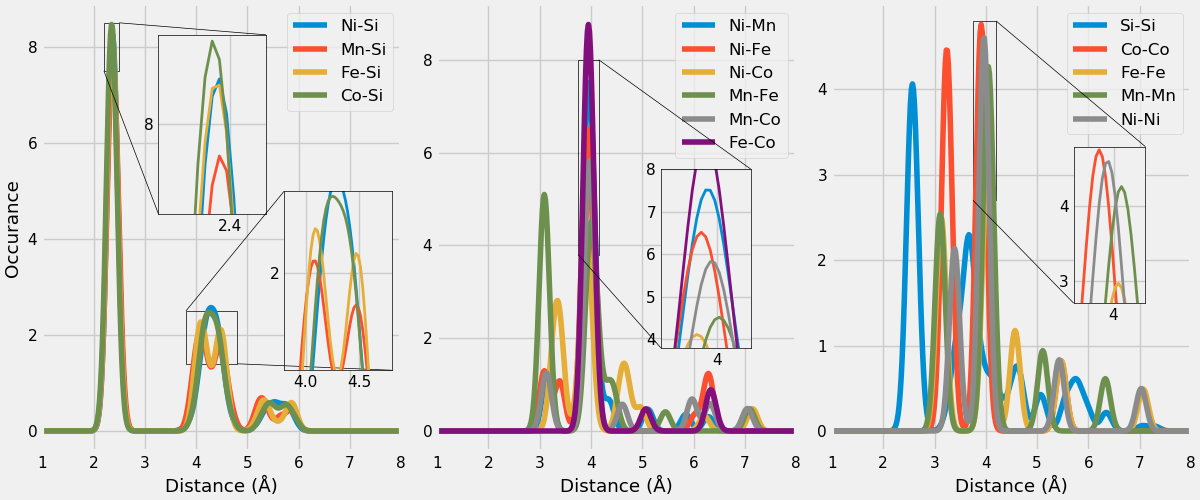
\includegraphics[width=\textwidth]{results/fesi2/composistions/cofemnni_PDF.png}
	\end{subfigure}
	\begin{subfigure}{\textwidth}
		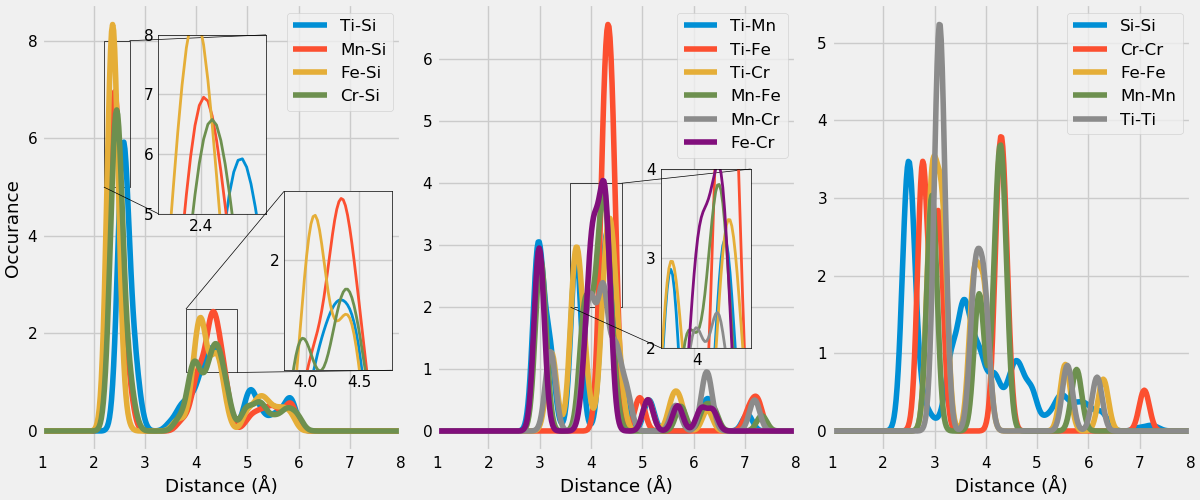
\includegraphics[width=\textwidth]{results/fesi2/composistions/crfemnti_PDF.png}
	\end{subfigure}
	\caption{Probability distribution function of \ch{Co4Fe4Mn4Ni4Si32} (top) and \ch{Cr4Fe4M4Ti4Si32} (bottom)}
\end{figure}

In regards to the band gap of the compositions, we can report that a heavy majority are metals. We found no evidence of a band gap in both the CrFeCoNiSi2 and CrFeMnTiSi2 alloys across all supercells, as seen in the density of states of the two most stable SQSs of the respective compounds \textbf{Add figures}. Further also the most stable SQSs of the CrFeTiNiSi alloy point to a metal. Similarly the most stable SQSs of the CoFeMnNiSi2 alloy are clearly metals. Noteworthy of this composition however is that we find clear evidence of a narrow band gap in two SQSs (A and B). In terms of stability, these lie around the mean total energy of the set. The respective band gaps are 0.033 eV in A and 0.0058 eV in B. \textbf{Include DOS or other figures for these results.} 

\begin{figure}[H]
\hskip-5cm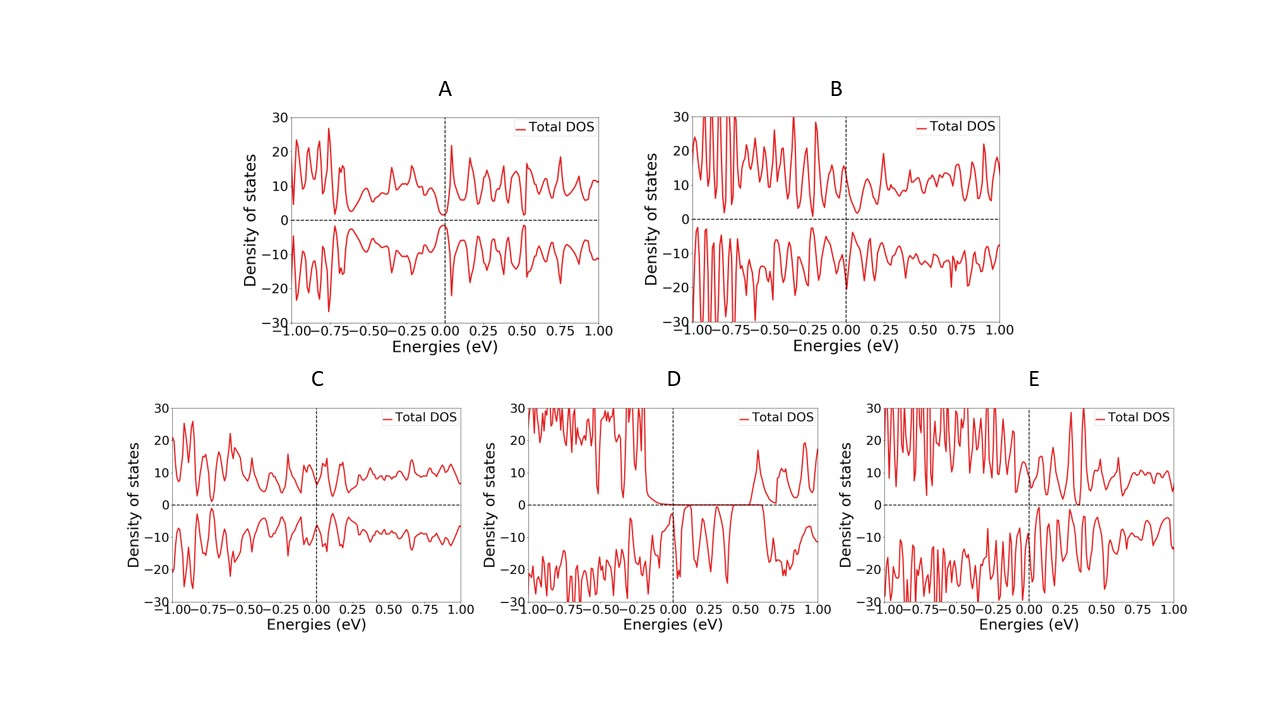
\includegraphics[scale=.65]{results/fesi2/composistions/all_DOS.jpg}
\caption{Density of states of A: \ch{CrFeCoNiSi2}, B: \ch{CrFeTiNiSi2}, C: \ch{CoFeMnNiSi2}, D: \ch{CrFeMnCoSi2}, E: \ch{CrFeMnTiSi2}. Calculations performed with PBE GGA.}
\end{figure}


\textbf{To follow is details on the gaps in A and B, is it worth to include this?}
In the density of states plotted in figure .., the band gap in A is clearly visible. On the other hand the very narrow gap in B is not as apparent, as the states around Ef contain very small nonzero values.  This could be related to the low resolution of 2500 points in the density of states as seen before, especially considering the size of the gap. In opposite to the CFMN calculations previous we here experience excellent cohesion between PBE and SCAN simulations on the band gap. With the meta-GGA functional the band gap of SQS A and B respective is 0.04 eV and the 0.003 eV. Moreover we find the identical gap transition with both functionals, which was not the case in previous endeavors with this functional. Additionally we also find that the HSE06 functional produce dissimilar results to previous experiences. In this scenario, the HSE06 functional fails to recognize the observed band gap of PBE and SCAN in both supercells. The greater number of k-points in the GGA and meta-GGA calculations offer more accurate band gaps, however lesser k-points will not result in a smaller gap, only bigger. Thus the uncertainties of previous calculations of the HSE06 functional does not apply in this case. For this reason in addition to the reputation of hybrid functionals and the lack of other factors to negatively affect the validity of the result, we find it challenging to conclude on the band gap of these structures between functionals.

\section{Crystal structures}

In the discussion above we have covered in great detail the possibilites of high-entropy silicides based on the $\beta-$ \ch{FeSi2} unit cell with twice as many silicon atoms to 3d elements. The primary outcome and conclsion of this research was that particularly the combination of Cr, Fe, Mn and Ni resulted in superiour properties in the light of the motivatian behind this project. The next question we wish to answer is if ihe promising results of the CFMN system be reproduced in other symetries. In this section we will implement the CFMN composistion in crystal structures based on hexagonal \ch{CrSi2} ($P6_{42\Bar{2}}$), both tetragonal and orthorombic \ch{Mn16Si28} ($P\Bar{4}c2 and$, $Pcca$), and trigonal \ch{Fe2Si} ($P\Bar{3}m1$) where we test the CFMN system to varying metal and silicon ratioes, and crystal structures. As before, the total energy, enthalpy of formation and magnetic moment per atom can be found bellow in table ..
\begin{table}[h!]
\begin{tabular}{@{}cccccc@{}}
\toprule
            & \multicolumn{2}{c}{Total energy per energy} & Enthalpy of formation & \multicolumn{2}{c}{Mag per atom} \\ \midrule
CrSi2       & -6.4837               & 0.0087              & -8.1205             & 0.0887          & 0.0387         \\
MnSi        & -6.6658               & 0.0071              & -9.1848             & 0.0687          & 0.0398         \\
Fe2Si       & -7.5082               & 0.0107              & -10.2474            & 0.3848          & 0.0588         \\ \bottomrule
\end{tabular}
\end{table}

\textbf{CrSi2 \\}
From our calculations with PBE DFT we find the bulk crsi2 material to be an indirect semiconductor with a band gap of 0.33 eV, slightly bellow the listed value of 0.36 eV in materials project \textbf{cite}, suprinsingly we find a smaller gap of 0.32 eV from the SCAN functional. The compound is also nonmagnetic in agreement with materials project. Fore the bulk material we employed a 9 atom cell, with 6 silicon and 3 cr atoms, from this we generated SQSs of 72 atoms with the same ratio.  \textbf{Include toten per atom for the unit cell? and figure of SQS + unit cell?}. For this given composistion and system we observe very similar results to that of the composistions discussed above, the eigenvalues of several SQSs report a small band gap, but its not apperant from neither the density of states or from the bandgap.py script of pymatgen. Additiontly, we can not repreoduce the gap with the SCAN functional, as was possible for the CFMN (fesi2) system.   

\paragraph{MnSi \\}
In the tetragonal configuration, the bulk material is a nonmagnetic indirect semiconductor with a band gap of 0.76 eV acoording to our PBE calculations,  and 0.78 eV from SCAN. Materials project find a band gap of 0.76 eV, in good agreement with our own PBE results. The unit cell consist of 44 total atoms, 16 manganese and 28 silicon. In the orthoromibic cell, with equal number of elements we find a band gap of 0.76 eV (0.77 ev SCAN) as well. In contrast, the CFMN alloy of both these cells produce metalic compounds. It should be noted that structures B and D in the tetragonal ssystem did not fully relax, same for D in the orthorombic cell, so these results could be inaccurate.   

\paragraph{Fe2Si \\}
In this cell, we drasticly alter the metal-silicon ratio, this is seen both in the band gap and magnetic properties of the material. The magnetic moment of this cell consisting of 4 iron atoms and 2 silicon atoms is 0.67, from the iron atoms. This magnetic charachter can also be observed from the discrepency between the two spin channels. In spin down we find a band gap of 0.21 eV, while there is no gap in spin up. This gap can also be seen in the density of states \textbf{Include figure}. This however is an abnormal result in regard to other experimental work and littereature on the Fe2Si \textbf{cite $https://www.sciencedirect.com/science/article/pii/S0925838816329796?casa_token=g9DRpU9IClcAAAAA:6Gd12A4Kh9J2igUWMVwHN8OSIKzD27VACA052FNsSAWhRY6PELWdVEPbiF8OtQ3eJEAbvQ8X0g$}. Our results are subject to errors, particularly we note that the eigenvalues used to calculate the gap contain nonphysical values in the spin down channel. However, the gap is evident in the density of states thus we include the result in this report, but acknowlendge the uncertainties revolving the value. 

From this unit cell we generate 54 atom SQSs. From table .. we see that the magnetic nature remains, producing the overall highest magnetic moment of all studied supercells, which is not a surprising result considering the 3d metal to silicon ratio. \textbf{More on magnetic and total energy.} The magnetism can also be seen in the difference between the two spin channels, the bands where the occupancy transistion from 1 to 0, ie occupied to not occupied is very different. In the most magnetic supercell D, we saw a distance of 22 bands between the spin down transistion and spin down transistion. Most supercells are metals from our PBE calculations. B and D show a very small gap of around 0.01 eV in one spin channel.  In E we find a very narrow gap semiconductor with a total gap of 0.002 eV. This gap is surrounded by the same uncertainties as discussed previosly.
